\chapter{\IfLanguageName{dutch}{Stand van zaken}{State of the art}}%
\label{ch:stand-van-zaken}

% Tip: Begin elk hoofdstuk met een paragraaf inleiding die beschrijft hoe
% dit hoofdstuk past binnen het geheel van de graduaatsproef. 
% Geef in het bijzonder aan wat de link is met het vorige en volgende hoofdstuk.

% Pas na deze inleidende paragraaf komt de eerste sectiehoofding.

% Dit hoofdstuk bevat je literatuurstudie.
% De inhoud gaat verder op de inleiding, maar zal het onderwerp van de graduaatsproef *diepgaand* uitspitten.
% De bedoeling is dat de lezer na lezing van dit hoofdstuk helemaal op de hoogte is van de huidige stand van zaken (state-of-the-art) in het onderzoeksdomein.
% Iemand die niet vertrouwd is met het onderwerp, weet nu voldoende om de rest van het verhaal te kunnen volgen, zonder dat die er nog andere informatie moet over opzoeken.

% Je verwijst bij elke bewering die je doet, vakterm die je introduceert, enz.\ naar je bronnen. 
% In \LaTeX{} kan dat met het commando \texttt{$\backslash${textcite\{\}}} of \texttt{$\backslash${autocite\{\}}}. 
% Als argument van het commando geef je de ``sleutel'' van een ``record'' in een bibliografische databank in het Bib\LaTeX{}-formaat (een tekstbestand). 
% Als je expliciet naar de auteur verwijst in de zin (narratieve referentie), gebruik je \texttt{$\backslash${}textcite\{\}}. 
% Soms is de auteursnaam niet expliciet een onderdeel van de zin, dan gebruik je \texttt{$\backslash${}autocite\{\}} (referentie tussen haakjes). 
% Dit gebruik je bv.~bij een citaat, of om in het bijschrift van een overgenomen afbeelding, broncode, tabel, enz. te verwijzen naar de bron. 
% In de volgende paragraaf een voorbeeld van elk.

% \textcite{Knuth1998} schreef een van de standaardwerken over sorteer- en zoekalgoritmen.
% Experten zijn het erover eens dat cloud computing een interessante opportuniteit vormen, 
% zowel voor gebruikers als voor dienstverleners op vlak van informatietechnologie~\autocite{Creeger2009}.

% Let er ook op: het \texttt{cite}-commando voor de punt, dus binnen de zin.
% Je verwijst meteen naar een bron in de eerste zin die erop gebaseerd is, dus niet pas op het einde van een paragraaf.


This section will review information on cross-platform technologies and help justify the selection of technology for the proof-of-concept application. Like the mobile smartphones the idea of cross-platform development is relatively young, so it should not be surprising that most publications on this topic come from the last few years. For the purposes of this work, mainly online articles, documentation of frameworks and coding languages have been analyzed. There are many solutions for cross-platform software development, here will be the most popular described. The purpose of the literature review is to compare the technologies in terms of available platforms, for which applications can be published, level of difficulty and complexity of the developement process.


\section{{Flutter}}%
\label{sec:flutter}

Flutter is one of the most popular cross-platform frameworks. It was weleased by Google in 2017 and uses Dart as its programming language and offers a rich set of pre-built widgets.
The framework privides a 'hot reload' feature what allows developers to see how the application looks as soon as code changes without recompiling. It supports Google's Material Design and doesn't rely on web browser technology. Instead, it has its own rendering engine for drawing widgets \autocite{FlutterDoc}.

\section{{React Native}}%
\label{sec:reactnative}

React Native is an open-source framework developed by Facebook (now Meta) for building cross-platform mobile apps using React, a JavaScript library. It allows developers already familiar with  web-development technologies to create native mobile applications for iOS and Android using a single codebase. It provides a set of pre-built components that can be used to create user interfaces, such as buttons, text fields, and views. The developing principles are very similar to React web-framework, orginal html tags were replaced with dedicated components like <Text> or <TouchableOpacity> \autocite{ReactNative}. React Native is one of the most popular framework for mobile development with great support of developers community.

It runs in a background process interpreting the JavaScript code directly on the target device and communicates with the native platform using serialized data over an asynchronous bridge \autocite{ReactNativeMedium}. Hot reload feature is also available.

According to the article written by Radhika Vyas  in 'Index.dev', React Native is efficient, but its performance lags below native apps, especially in sophisticated apps needing significant computations or animations. It also has problems with achieving a uniform look and feel across both iOS and Android may be difficult and requires more work to satisfy users experience, \textcite{Vyas}.

Publishing React Native projects as Web Apps is also possible, but can be difficult due to incompatibility of components between web-browser and mobile device, what requires platform specific conditional component rendering.



\begin{listing}[H]
\begin{minted}{react}
<View>
    {Platform.OS == "android" || Platform.OS == "ios" ? (
        <DatePicker modal open={visibleDatePicker} mode="date" date={date}
            onConfirm={(date) => {
                onDateOK(date);
                }}
            onCancel={() => {
                setDatePickerVisible(false);
                }}
        />) : (
        <DatePickerModal label="Choose date" date={date}
            mode="single" saveLabel="Ok" visible={visibleDatePicker}
            onDismiss={() => {
                    setDatePickerVisible(false);
                }}
            onConfirm={(params) => {
                    if (params.date) onDateOK(params.date);
                    setDatePickerVisible(false);
                }}
        />
    )}
</View>
\end{minted}
\caption[React Native platform specific conditional rendering]{React Native platform specific conditional rendering. Example provided by thesis author uses two different components depending on target OS}
\end{listing}
                

\section{{Cordova}}
\label{sec:cordova}
Cordova is an open-source mobile development framework maintained by Apache Software Foundation which allows using standard web technologies like HTML, CSS, and JavaScript for mobile cross-platform development \autocite{CordovaDoc}. To implement mobile platform sppecific native features developers can use plugins like battery status, camera access, native dialogs, screen orientation,vibration or geolocation. Cordova contains several components, the following diagram shows a high-level view of its system architecture.

\begin{figure}[H]
    \centering
    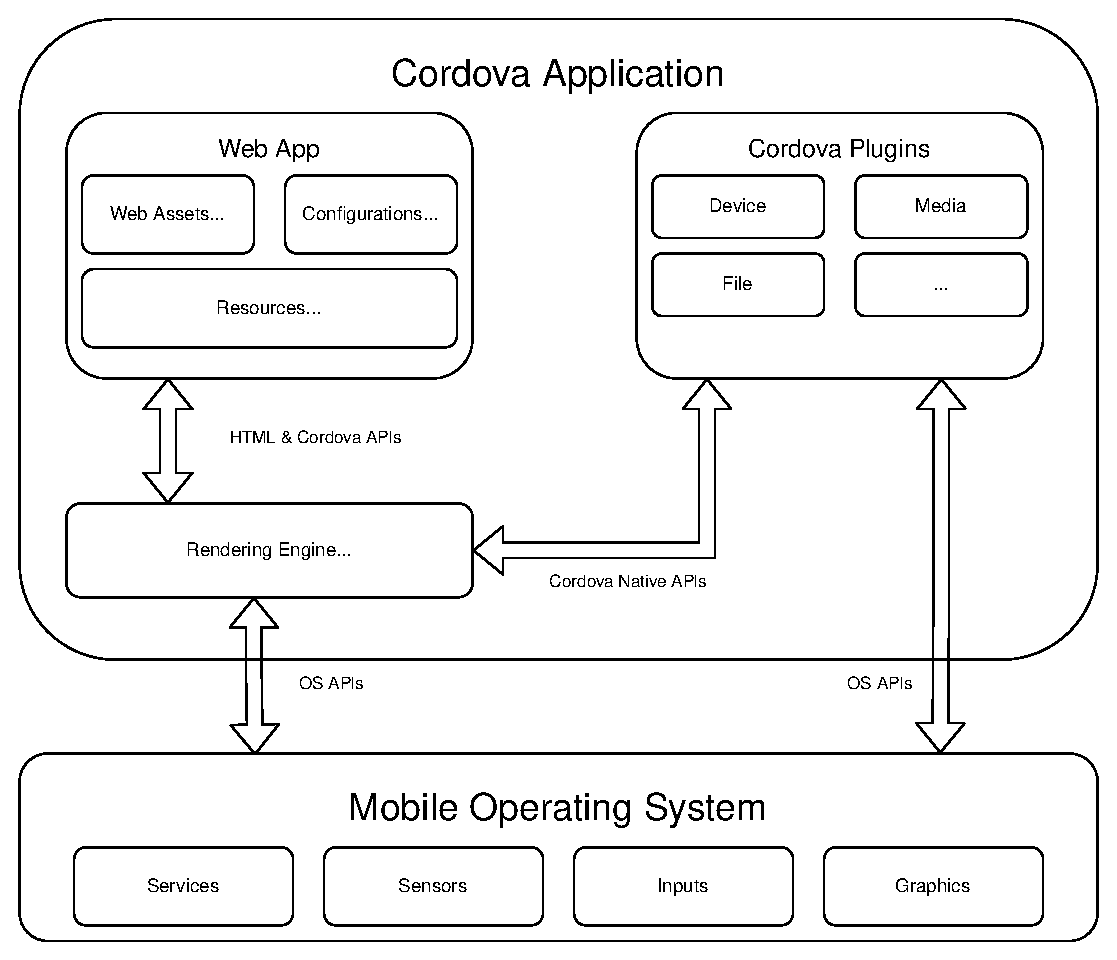
\includegraphics[width=0.6\textwidth]{cordova_arch.eps}
    \caption[Cordova architecture]{\label{fig:cordova} Cordova architecture }
\end{figure}    
                
\section{{Ionic}}%
\label{sec:ionic}

Ionic Framework is an open-source mobile app development platform that allows developers to build native and progressive web apps with web technologies such as HTML, CSS, and JavaScript. It is built on top of the Angular and Cordova frameworks. It can be combined with JavaScript-based web frameworks like React and Vue.

Regarding the previously cited article from Radhika Vyas in 'Index.dev',
\begin{displayquote}
Ionic's dependence on well-known web technologies makes it easily accessible to web developers, therefore enabling them to move naturally into mobile development, but: \newline
% \end{displayquote}
% , but also:
% \begin{displayquote}
    As Ionic depends on web technologies instead of native code, it might suffer from speed problems in graphics-intensive apps even if it is appropriate for most uses. Accessing native functionality often calls for plugins, which might cause extra complexity and sometimes compatibility problems, \textcite{Vyas}.
\end{displayquote}




\section{{MAUI .NET}}%
\label{sec:maui}

For developers who prefer to code in .NET environment, Microsoft offers a Multi-platform App UI (.NET MAUI), a framework for creating native mobile and desktop apps that can run on Android, iOS, macOS, and Windows from a single shared code-base written with C\# and XAML  \autocite{XAML} \autocite{MAUIDocs}. MAUI is an evolution of its predecessor - Xamarin.Forms \autocite{Xamarin} and provides a single framework for building the UIs for mobile and desktop environment. The following diagram demonstrates the architecture of a .NET MAUI App:

\begin{figure}[H]
    \centering
    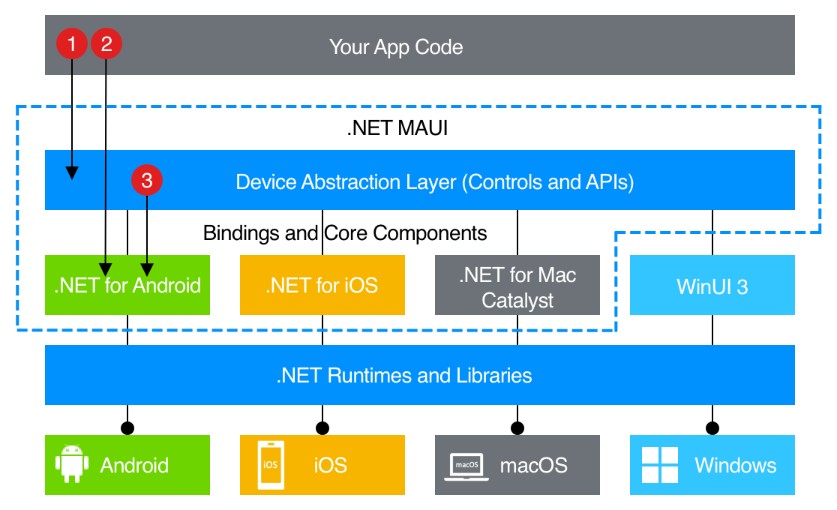
\includegraphics[width=0.8\textwidth]{maui-diagram.png}
    \caption[MAUI architecture]{\label{fig:maui} In a .NET MAUI app, written code interacts primarily  with the .NET MAUI controls and API layer (1). This layer then directly consumes the native platform APIs (3). In addition, app code may directly exercise platform APIs (2), if required. \autocite{MAUIDocs}}
\end{figure}

.NET MAUI projects can be written on Windows PC (Visual Studio or vscode) or Mac (vscode, JetBrains Rider \autocite{JBrainsRider}), and compiled into native app packages.
It also  provides APIs for native device features like access to sensors, such as the accelerometer, compass, and gyroscope on devices, ability to check the device's network connectivity state, picking files from the device, store data and initiate browser-based authentication. MAUI includes support for 'hot reload' technique, which allows code modifications on running app, without the need to recompile. 




\section{{Tauri}}%
\label{sec:tauri}

The youngest open-source framework in this comparison is Tauri. It's designed to create projects for all popular operating systems: Linux, macOS, Windows, Android and iOS using a local device WebView \autocite{WebView} frontend libraries and a Rust language \autocite{RustWiki} sourced binary back-end with an API that the front-end can interact with. Tauri uses web technologies that means that virtually any frontend framework is compatible. Technically, the presentation layer is managed by two librieries: TAO - responsible for Tauri window creation and WRY - responsible for web view rendering \autocite{TauriDoc}. 

\begin{figure}[H]
    \centering
    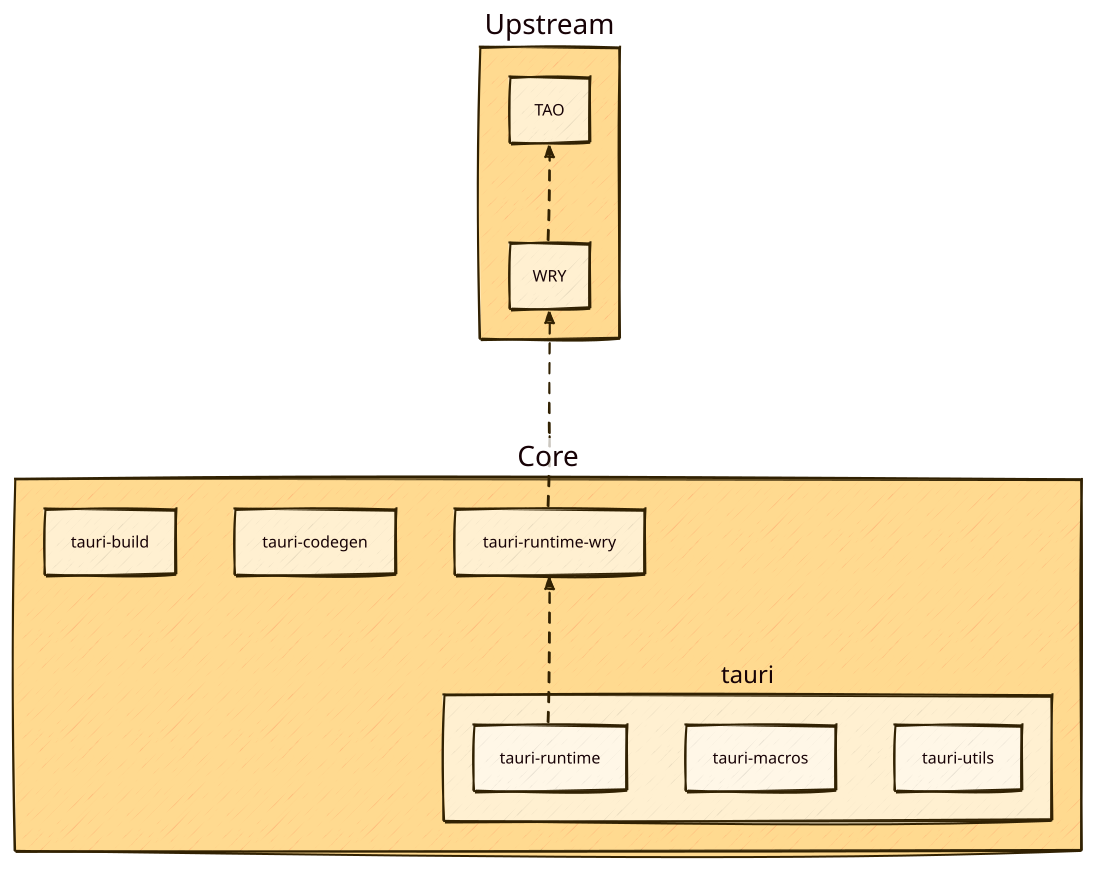
\includegraphics[width=0.6\textwidth]{tauri-arch.png}
    \caption[Tauri architecture]{\label{fig:tauri} Tauri architecture diagram }
\end{figure}


\section{{Electron}}%
\label{sec:electron}
Electron is a framework for building desktop applications for Windows, macOS, and Linux using Web technologies like JavaScript, HTML, and CSS. It is based on Google Chromium Web browser and Node.js in its binary, Electron allows developers to maintain one single JavaScript codebase and publish everywhere without native development experience required \autocite{ElectronDoc}.

Many worldwide popular desktop applications are build with Electron framework: Visual Studio Code \autocite{Vscode}, Signal \autocite{Signal}, Discord, Postman \autocite{Postman}, ... and many others including Mediko - a proof-of-concept application written for the purpose of this thesis \ref{sec:desktop}.

\begin{figure}[H]
    \centering
    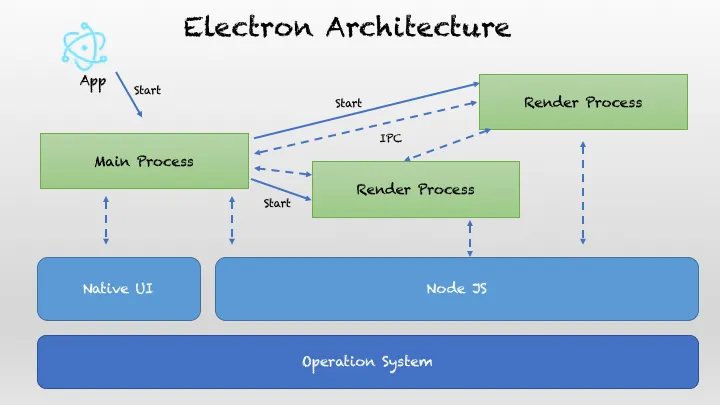
\includegraphics[width=0.6\textwidth]{electron-arch.png}
    \caption[Electron architecture]{\label{fig:electronarch} Electron architecture \autocite{ElectronArch} }
\end{figure}



\section{{Summary}}%
\label{sec:literature_summary}

After analyzing the literature, the following conclusions may be drawn:
\begin{itemize}
    \item JavaScript seems to be the most universal programming language
    \item web-based framework can provide opportunity for most efficient development process
\end{itemize}

It is also possible to use multiple technologies in one project, for examplpe SPA web application build on Vue, React or Angular for online web pages, Cordova or Tauri to publish mobile application and Electron for desktop environments. 
What is worth of noting, all of the analyzed frameworks are open-source, which illustrates trends in today's computer science.


\begin{table}[H]
    \centering
    \begin{tabular}{lcccccc}
      \toprule
                        & Windows &  macOS  & Linux &  iOS  & Android &  Web  \\
      \midrule
      Flutter (Dart)    &   yes   &   yes   &  (4)  &  yes  &   yes   &  yes  \\
      React Native (JS) &   (2)   &   (3)   &  (3)  &  yes  &   yes   &  yes  \\
      Cordova (JS)      &   (1)   &   (1)   &  (1)  &  yes  &   yes   &  yes  \\
      Ionic (JS)        &   (1)   &   (1)   &  (1)  &  yes  &   yes   &  yes  \\
      .NET MAUI (C\#)   &   yes   &   yes   &   -   &  yes  &   yes   &   -   \\
      Tauri (JS, Rust)  &   yes   &   yes   &  yes  &  yes  &   yes   &  yes  \\
      Electron (JS)     &   yes   &   yes   &  yes  &  -    &    -    &  -    \\
      \bottomrule
    \end{tabular}
    \caption[Platform availability]{\label{tab:example}Target platform availability depending on frameworks.
    \newline ( 1 ) by adding Electron package
    \newline ( 2 ) via React Native Skia as a renderer Out-of-Tree Platform.
    \newline ( 3 ) React Native for Microsoft's Universal Windows Out-of-Tree Platform
    \newline ( 4 ) officially only for Debian/Ubuntu
    }
  
\end{table}